\section{Self-Adaptive Systems}

Self-adaptivesses is an approach in which the system
\emph{"evaluates its own behavior and changes behavior when the evaluation indicates that it is not accomplishing what the software is intended to do, or when better functionality or performance is possible."}\cite{laddaga_self_1997}.
Self-adaptive systems (SAS) aims to adjust various artifacts or attributes in response to changes in the self and in the context of a software system\cite{salehie_self-adaptive_2009}.

A key concept in self-adaptive systems is the awareness of the system. It has two aspects\cite{salehie_self-adaptive_2009}:
\begin{itemize}
   \item \emph{context-awareness} means that the system is aware of its context.
   \item \emph{self-awareness} means a system is aware of its own states and behaviors.
\end{itemize}

Schilit et al.\cite{klein_survey_2008} define \emph{context adaptation} as \say{a system’s capability of gathering information about the domain it shares an interface with, evaluating this information and changing its observable behavior according to the current situation}.

\begin{figure}[!htb]
 \centering
 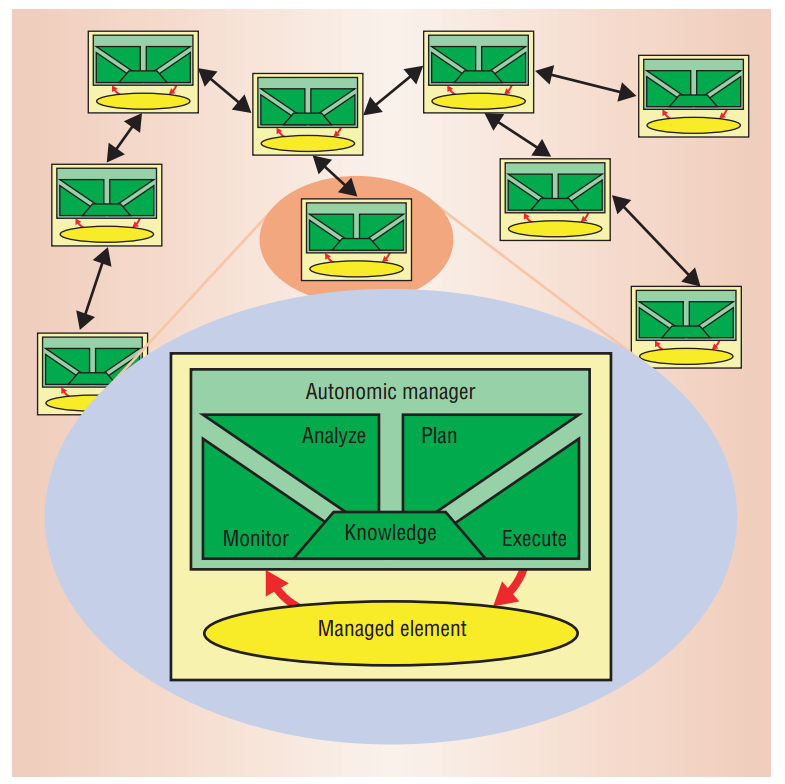
\includegraphics[width=0.7\linewidth]{mape-k}
 \caption{MAPE-K Reference Architecture}
\label{fig:mape-k}
\end{figure}

MAPE-K is a reference architecture originally proposed for autonomic computing~\ref{kephart_vision_2003} and that is often used as a model for architectures of SAS. It has a control loop, realized by a simple sequence of four activities: \emph{monitor}, \emph{analyze}, \emph{plan}, and \emph{execute}. Where monitoring collects data from \emph{sensors}, while executing is done through \emph{actuators}. In addition, all activities can share information throught a \emph{knowledge} system.

\subsection{Development of Self-Adaptive Systems}

For SAS some activities that traditionally occur at development-time are moved to runtime.  In~\cite{andersson_software_2013}
was proposed a process for development of adaptive systems.
Activities performed externally are referred as \emph{off-line activities}, and activities performed internally as \emph{on-line activities}.


\begin{figure}[!htb]
  \centering
  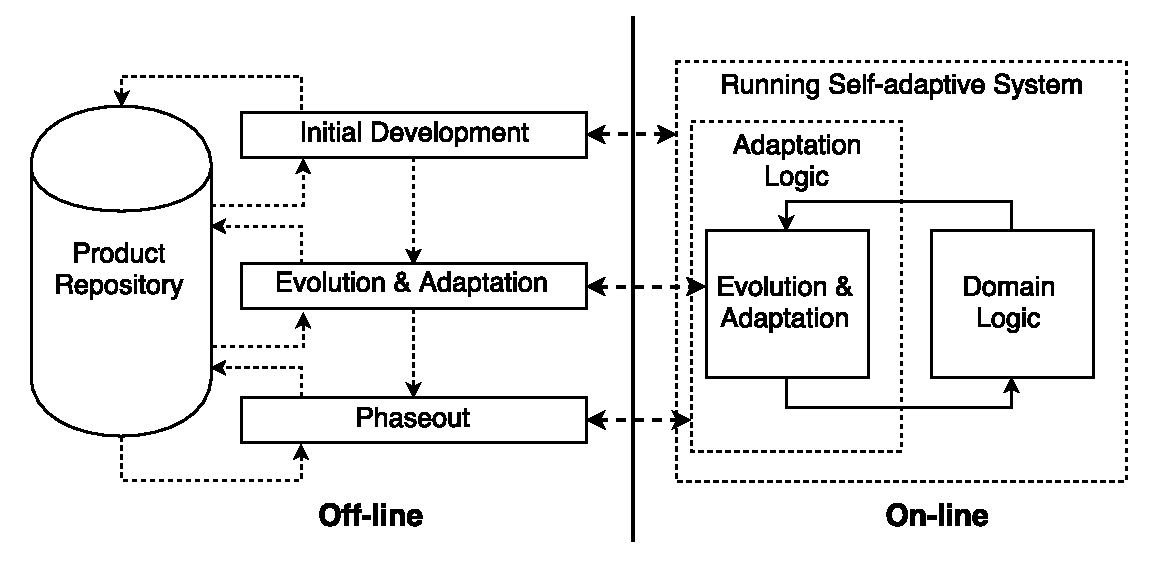
\includegraphics[width=\linewidth]{sas_lifecycle}
  \caption{A Life-cycle model for Self-Adaptation Software System\cite{andersson_software_2013}}
  \label{fig:sas_lifecycle}
\end{figure}

The right-hand side of Figure~\ref{fig:sas_lifecycle} depicts a running SAS. At this system we have \emph{Domain Logic} that solves that is responsible for final user goals achievements. And also, \emph{Adaptation Logic}, that is responsible to adapt the system in response to changes in the environment. Adaptation logic implements a control loop in line with the monitor-analyze-plan-execute (MAPE) loop~\cite{kephart_vision_2003}.

The left-hand side of Figure~\ref{fig:sas_lifecycle} represents a staged life-cycle model. Off-line activities work on artifacts such as design model and source code in a product repository and not directly on the running system.
